\documentclass[11pt, letterpaper]{article}

% Fonts and Encoding
\usepackage[utf8]{inputenc}
\usepackage[T1]{fontenc}
\usepackage{lmodern}

% Math and Symbols
\usepackage{amsmath, amssymb, amsthm, amsfonts, mathrsfs, mathtools}

% Layout and Geometry
\usepackage{geometry}
\geometry{letterpaper, margin=1in}
\setlength{\parindent}{0pt}
\setlength{\parskip}{0.6em}

% Formatting and Graphics
\usepackage{graphicx, xcolor, enumitem, booktabs, array, tabularx}

% TikZ for Illustrations
\usepackage{tikz}
\usetikzlibrary{arrows.meta, positioning, shapes.geometric, calc, backgrounds, matrix}

% Clickable Links and TOC
\usepackage{hyperref}
\hypersetup{
    colorlinks=true,
    linkcolor=blue,
    filecolor=magenta,      
    urlcolor=cyan,
    pdftitle={Advanced Mathematics Topic},
}

% Theorem Environments
\newtheorem{theorem}{Theorem}[section]
\newtheorem{lemma}[theorem]{Lemma}
\newtheorem{proposition}[theorem]{Proposition}
\newtheorem{corollary}[theorem]{Corollary}
\theoremstyle{definition}
\newtheorem{definition}{Definition}[section]
\newtheorem{axiom}{Axiom}[section]
\newtheorem{example}{Example}[section]
\theoremstyle{remark}
\newtheorem{remark}{Remark}[section]

% Custom Commands (Enforced standard notation)
\newcommand{\R}{\mathbb{R}}
\newcommand{\N}{\mathbb{N}}
\newcommand{\Z}{\mathbb{Z}}
\newcommand{\Q}{\mathbb{Q}}
\newcommand{\E}{\mathbb{E}}
\newcommand{\Prob}{\mathbb{P}}
\newcommand{\F}{\mathcal{F}}

\title{\Huge \textbf{Mastering Complex Eigenvalues} \\ \Large A Comprehensive Guide to Rotations, Scaling, and Invariant Subspaces}
\author{Tashfeen Omran}
\date{\today}

\begin{document}

\maketitle
\tableofcontents
\newpage

\section{Comprehensive Introduction, Context, and Prerequisites}

\subsection{Core Concepts}
In the study of linear algebra, the characteristic equation of an $n \times n$ matrix $A$, given by $\det(A - \lambda I) = 0$, is a polynomial of degree $n$. By the Fundamental Theorem of Algebra, this polynomial always has exactly $n$ roots (counting multiplicities) over the complex numbers, $\mathbb{C}$. When a real matrix $A$ has complex eigenvalues, they always occur in conjugate pairs: $\lambda = a \pm bi$. 

Corresponding to these complex eigenvalues are complex eigenvectors. If $\mathbf{v}$ is an eigenvector for $\lambda = a - bi$, then its complex conjugate $\bar{\mathbf{v}}$ is an eigenvector for $\bar{\lambda} = a + bi$. The presence of complex eigenvalues in a real matrix indicates that the linear transformation $\mathbf{x} \mapsto A\mathbf{x}$ involves a rotational component, often combined with scaling.

\subsection{Intuition and Derivation}
Why do we care about complex eigenvalues for real matrices? In $\R^2$, a matrix with complex eigenvalues does not simply stretch vectors along fixed lines (as real eigenvalues do). Instead, it rotates them. 

Consider a complex eigenvalue $\lambda = a - bi$ and its corresponding eigenvector $\mathbf{v} = \text{Re}(\mathbf{v}) + i\text{Im}(\mathbf{v})$. By separating the real and imaginary parts of the equation $A\mathbf{v} = \lambda\mathbf{v}$, we can construct a real $2 \times 2$ matrix $P = [\text{Re}(\mathbf{v}) \quad \text{Im}(\mathbf{v})]$. This matrix $P$ acts as a change of basis, transforming $A$ into a special block matrix $C$:
\[
A = PCP^{-1} \quad \text{where} \quad C = \begin{bmatrix} a & -b \\ b & a \end{bmatrix}
\]
The matrix $C$ is a pure rotation combined with a scaling. By factoring out $r = \sqrt{a^2 + b^2}$, we get $C = r \begin{bmatrix} \cos\phi & -\sin\phi \\ \sin\phi & \cos\phi \end{bmatrix}$, which clearly shows a rotation by angle $\phi$ and a scaling by factor $r$.

\subsection{Historical Context and Motivation}
The study of complex eigenvalues arose from the need to understand dynamical systems, periodic motion, and vibrations in physics and engineering. In the 19th century, mathematicians like Augustin-Louis Cauchy and Karl Weierstrass formalized eigenvalue theory to solve systems of linear differential equations. When modeling a pendulum, an electrical circuit, or planetary orbits, the state variables often oscillate. These oscillations are mathematically captured by the imaginary components of complex eigenvalues, which dictate the frequency of rotation in the system's phase space.

\subsection{Key Formulas}
\renewcommand{\arraystretch}{1.5}
\begin{tabularx}{\textwidth}{>{\raggedright\arraybackslash}X >{$\displaystyle}c<{$} >{$\displaystyle}c<{$}}
\toprule
\textbf{Concept} & \textbf{Formula} & \textbf{Description} \\
\midrule
Characteristic Equation & \det(A - \lambda I) = 0 & Used to find eigenvalues $\lambda$. \\
\addlinespace[4pt]
Complex Eigenvalue & \lambda = a - bi & Standard form for factorization. \\
\addlinespace[4pt]
Rotation-Scaling Matrix & C = \begin{bmatrix} a & -b \\ b & a \end{bmatrix} & The hidden rotation inside $A$. \\
\addlinespace[4pt]
Change of Basis Matrix & P = [\text{Re}(\mathbf{v}) \quad \text{Im}(\mathbf{v})] & Maps the standard basis to the rotation basis. \\
\addlinespace[4pt]
Scale Factor & r = |\lambda| = \sqrt{a^2 + b^2} & The amount the vector is stretched. \\
\addlinespace[4pt]
Rotation Angle & \phi = \arctan\left(\frac{b}{a}\right) & The angle of rotation (adjust for quadrant). \\
\bottomrule
\end{tabularx}

\subsection{Prerequisites}
To master this topic, you must be proficient in:
\begin{itemize}
    \item \textbf{Determinants and Characteristic Equations:} Computing $\det(A - \lambda I)$ for $2 \times 2$ and $3 \times 3$ matrices.
    \item \textbf{Complex Arithmetic:} Adding, multiplying, and finding the conjugate of complex numbers ($i^2 = -1$).
    \item \textbf{Null Spaces:} Solving $(A - \lambda I)\mathbf{x} = \mathbf{0}$ using row reduction or substitution.
    \item \textbf{Trigonometry:} Understanding polar coordinates, $\sin\phi$, and $\cos\phi$.
\end{itemize}

\newpage

\section{Detailed Homework Solutions}
\textit{Note: A strategic selection of problems has been chosen to cover every distinct problem archetype present in the text, ensuring comprehensive mastery without redundant repetition.}

\subsection{Archetype 1: Finding Complex Eigenvalues and Eigenvectors}

\textbf{Problem 1:} Let $A = \begin{bmatrix} 1 & -2 \\ 1 & 3 \end{bmatrix}$ act on $\mathbb{C}^2$. Find the eigenvalues and a basis for each eigenspace in $\mathbb{C}^2$.

\textbf{Solution:}
First, we find the characteristic equation $\det(A - \lambda I) = 0$:
\[
\det \begin{bmatrix} 1 - \lambda & -2 \\ 1 & 3 - \lambda \end{bmatrix} = (1 - \lambda)(3 - \lambda) - (-2)(1) = 0
\]
\[
\lambda^2 - 4\lambda + 3 + 2 = \lambda^2 - 4\lambda + 5 = 0
\]
Using the quadratic formula:
\[
\lambda = \frac{4 \pm \sqrt{16 - 20}}{2} = \frac{4 \pm \sqrt{-4}}{2} = \frac{4 \pm 2i}{2} = 2 \pm i
\]
The eigenvalues are $\lambda_1 = 2 - i$ and $\lambda_2 = 2 + i$.

Next, we find the eigenvector for $\lambda_1 = 2 - i$:
\[
A - (2 - i)I = \begin{bmatrix} 1 - (2 - i) & -2 \\ 1 & 3 - (2 - i) \end{bmatrix} = \begin{bmatrix} -1 + i & -2 \\ 1 & 1 + i \end{bmatrix}
\]
We solve $(A - \lambda_1 I)\mathbf{x} = \mathbf{0}$. The two rows are linearly dependent over $\mathbb{C}$. Using the second row:
\[
1x_1 + (1 + i)x_2 = 0 \implies x_1 = -(1 + i)x_2
\]
Let $x_2 = 1$, then $x_1 = -1 - i$. The eigenvector is $\mathbf{v}_1 = \begin{bmatrix} -1 - i \\ 1 \end{bmatrix}$.
Since the matrix is real, the eigenvector for $\lambda_2 = 2 + i$ is the complex conjugate: $\mathbf{v}_2 = \begin{bmatrix} -1 + i \\ 1 \end{bmatrix}$.

\textbf{Final Answer:} 
Eigenvalues: $\lambda = 2 \pm i$. 
Basis for $\lambda = 2 - i$: $\left\{ \begin{bmatrix} -1 - i \\ 1 \end{bmatrix} \right\}$. 
Basis for $\lambda = 2 + i$: $\left\{ \begin{bmatrix} -1 + i \\ 1 \end{bmatrix} \right\}$.

\vspace{1em}

\textbf{Problem 4:} Let $A = \begin{bmatrix} -7 & 1 \\ -5 & -3 \end{bmatrix}$. Find the eigenvalues and a basis for each eigenspace.

\textbf{Solution:}
Characteristic equation:
\[
\det \begin{bmatrix} -7 - \lambda & 1 \\ -5 & -3 - \lambda \end{bmatrix} = (-7 - \lambda)(-3 - \lambda) - (-5)(1) = 0
\]
\[
\lambda^2 + 10\lambda + 21 + 5 = \lambda^2 + 10\lambda + 26 = 0
\]
Quadratic formula:
\[
\lambda = \frac{-10 \pm \sqrt{100 - 104}}{2} = \frac{-10 \pm 2i}{2} = -5 \pm i
\]
For $\lambda_1 = -5 - i$:
\[
A - (-5 - i)I = \begin{bmatrix} -2 + i & 1 \\ -5 & 2 + i \end{bmatrix}
\]
Using the first row: $(-2 + i)x_1 + x_2 = 0 \implies x_2 = (2 - i)x_1$.
Let $x_1 = 1$, then $x_2 = 2 - i$. The eigenvector is $\mathbf{v}_1 = \begin{bmatrix} 1 \\ 2 - i \end{bmatrix}$.
The conjugate eigenvector for $\lambda_2 = -5 + i$ is $\mathbf{v}_2 = \begin{bmatrix} 1 \\ 2 + i \end{bmatrix}$.

\textbf{Final Answer:} 
Eigenvalues: $\lambda = -5 \pm i$. 
Basis for $\lambda = -5 - i$: $\left\{ \begin{bmatrix} 1 \\ 2 - i \end{bmatrix} \right\}$. 
Basis for $\lambda = -5 + i$: $\left\{ \begin{bmatrix} 1 \\ 2 + i \end{bmatrix} \right\}$.

\subsection{Archetype 2: Geometric Interpretation (Rotation and Scaling)}

\textbf{Problem 7:} Use Example 6 to list the eigenvalues of $A = \begin{bmatrix} \sqrt{3} & -1 \\ 1 & \sqrt{3} \end{bmatrix}$. The transformation $\mathbf{x} \mapsto A\mathbf{x}$ is the composition of a rotation and a scaling. Give the angle $\phi$ of the rotation, where $-\pi < \phi \le \pi$, and give the scale factor $r$.

\textbf{Solution:}
The matrix is in the form $C = \begin{bmatrix} a & -b \\ b & a \end{bmatrix}$ with $a = \sqrt{3}$ and $b = 1$.
By Example 6, the eigenvalues are $\lambda = a \pm bi = \sqrt{3} \pm i$.
The scale factor is $r = |\lambda| = \sqrt{a^2 + b^2} = \sqrt{(\sqrt{3})^2 + 1^2} = \sqrt{4} = 2$.
The rotation angle $\phi$ satisfies $\cos\phi = \frac{a}{r} = \frac{\sqrt{3}}{2}$ and $\sin\phi = \frac{b}{r} = \frac{1}{2}$.
The angle in the first quadrant that satisfies these is $\phi = \frac{\pi}{6}$.

\textbf{Final Answer:} Eigenvalues: $\lambda = \sqrt{3} \pm i$. Scale factor $r = 2$. Angle $\phi = \frac{\pi}{6}$.

\vspace{1em}

\textbf{Problem 10:} Find the eigenvalues, angle $\phi$, and scale factor $r$ for $A = \begin{bmatrix} \sqrt{2} & -\sqrt{2} \\ \sqrt{2} & \sqrt{2} \end{bmatrix}$.

\textbf{Solution:}
Here, $a = \sqrt{2}$ and $b = \sqrt{2}$.
Eigenvalues: $\lambda = a \pm bi = \sqrt{2} \pm i\sqrt{2}$.
Scale factor: $r = \sqrt{(\sqrt{2})^2 + (\sqrt{2})^2} = \sqrt{2 + 2} = 2$.
Angle $\phi$: $\cos\phi = \frac{\sqrt{2}}{2}$ and $\sin\phi = \frac{\sqrt{2}}{2}$. This corresponds to $\phi = \frac{\pi}{4}$.

\textbf{Final Answer:} Eigenvalues: $\lambda = \sqrt{2} \pm i\sqrt{2}$. Scale factor $r = 2$. Angle $\phi = \frac{\pi}{4}$.

\subsection{Archetype 3: Matrix Factorization ($A = PCP^{-1}$)}

\textbf{Problem 13:} Find an invertible matrix $P$ and a matrix $C$ of the form $\begin{bmatrix} a & -b \\ b & a \end{bmatrix}$ such that $A = \begin{bmatrix} 1 & -2 \\ 1 & 3 \end{bmatrix}$ has the form $A = PCP^{-1}$.

\textbf{Solution:}
From Problem 1, we have $\lambda = 2 - i$ (so $a = 2, b = 1$).
The corresponding eigenvector is $\mathbf{v} = \begin{bmatrix} -1 - i \\ 1 \end{bmatrix}$.
We separate $\mathbf{v}$ into real and imaginary parts:
\[
\mathbf{v} = \begin{bmatrix} -1 \\ 1 \end{bmatrix} + i \begin{bmatrix} -1 \\ 0 \end{bmatrix} \implies \text{Re}(\mathbf{v}) = \begin{bmatrix} -1 \\ 1 \end{bmatrix}, \quad \text{Im}(\mathbf{v}) = \begin{bmatrix} -1 \\ 0 \end{bmatrix}
\]
We construct $P = [\text{Re}(\mathbf{v}) \quad \text{Im}(\mathbf{v})]$:
\[
P = \begin{bmatrix} -1 & -1 \\ 1 & 0 \end{bmatrix}
\]
The matrix $C$ is constructed using $a = 2$ and $b = 1$:
\[
C = \begin{bmatrix} a & -b \\ b & a \end{bmatrix} = \begin{bmatrix} 2 & -1 \\ 1 & 2 \end{bmatrix}
\]

\textbf{Final Answer:} $P = \begin{bmatrix} -1 & -1 \\ 1 & 0 \end{bmatrix}$ and $C = \begin{bmatrix} 2 & -1 \\ 1 & 2 \end{bmatrix}$.

\vspace{1em}

\textbf{Problem 16:} Find $P$ and $C$ for $A = \begin{bmatrix} -7 & 1 \\ -5 & -3 \end{bmatrix}$.

\textbf{Solution:}
From Problem 4, we have $\lambda = -5 - i$ (so $a = -5, b = 1$).
The corresponding eigenvector is $\mathbf{v} = \begin{bmatrix} 1 \\ 2 - i \end{bmatrix}$.
Separating into real and imaginary parts:
\[
\mathbf{v} = \begin{bmatrix} 1 \\ 2 \end{bmatrix} + i \begin{bmatrix} 0 \\ -1 \end{bmatrix} \implies \text{Re}(\mathbf{v}) = \begin{bmatrix} 1 \\ 2 \end{bmatrix}, \quad \text{Im}(\mathbf{v}) = \begin{bmatrix} 0 \\ -1 \end{bmatrix}
\]
Construct $P$:
\[
P = \begin{bmatrix} 1 & 0 \\ 2 & -1 \end{bmatrix}
\]
Construct $C$ using $a = -5$ and $b = 1$:
\[
C = \begin{bmatrix} -5 & -1 \\ 1 & -5 \end{bmatrix}
\]

\textbf{Final Answer:} $P = \begin{bmatrix} 1 & 0 \\ 2 & -1 \end{bmatrix}$ and $C = \begin{bmatrix} -5 & -1 \\ 1 & -5 \end{bmatrix}$.

\subsection{Archetype 4: Conceptual True/False}

\textbf{Problem 23:} (T/F) The matrix $A$ can have one real and one complex eigenvalue.

\textbf{Solution:}
\textbf{False.} If $A$ is a real matrix, its characteristic polynomial has real coefficients. By the Complex Conjugate Root Theorem, any complex roots must occur in conjugate pairs ($\lambda = a \pm bi$). Therefore, a $2 \times 2$ real matrix must have either two real eigenvalues or two complex eigenvalues.

\textbf{Problem 24:} (T/F) The points $A\mathbf{x}, A^2\mathbf{x}, A^3\mathbf{x}, \dots$ always lie on the same circle.

\textbf{Solution:}
\textbf{False.} The points lie on an ellipse, not necessarily a circle, because the basis vectors in $P$ may not be orthogonal or of equal length. Furthermore, they only lie on a closed loop if the scale factor $r = |\lambda| = 1$. If $r > 1$, the points spiral outward; if $r < 1$, they spiral inward toward the origin.

\subsection{Archetype 5: Theoretical Proofs}

\textbf{Problem 27:} Let $A$ be an $n \times n$ real matrix with the property that $A^T = A$. Let $\mathbf{x}$ be any vector in $\mathbb{C}^n$, and let $q = \bar{\mathbf{x}}^T A \mathbf{x}$. The equalities below show that $q$ is a real number by verifying that $\bar{q} = q$. Give a reason for each step.
\[
\bar{q} = \overline{\bar{\mathbf{x}}^T A \mathbf{x}} \overset{(a)}{=} \mathbf{x}^T \overline{A \mathbf{x}} \overset{(b)}{=} \mathbf{x}^T A \bar{\mathbf{x}} \overset{(c)}{=} (\mathbf{x}^T A \bar{\mathbf{x}})^T \overset{(d)}{=} \bar{\mathbf{x}}^T A^T \mathbf{x} \overset{(e)}{=} q
\]

\textbf{Solution:}
\begin{itemize}
    \item \textbf{(a)} The conjugate of a product is the product of the conjugates, and $\overline{\bar{\mathbf{x}}} = \mathbf{x}$.
    \item \textbf{(b)} Since $A$ is a real matrix, $\bar{A} = A$. Thus, $\overline{A\mathbf{x}} = \bar{A}\bar{\mathbf{x}} = A\bar{\mathbf{x}}$.
    \item \textbf{(c)} The quantity $\mathbf{x}^T A \bar{\mathbf{x}}$ is a $1 \times 1$ matrix (a scalar). The transpose of a scalar is itself.
    \item \textbf{(d)} The transpose of a product reverses the order: $(BC)^T = C^T B^T$. Here, $(\mathbf{x}^T (A \bar{\mathbf{x}}))^T = (A \bar{\mathbf{x}})^T (\mathbf{x}^T)^T = \bar{\mathbf{x}}^T A^T \mathbf{x}$.
    \item \textbf{(e)} By hypothesis, $A$ is symmetric ($A^T = A$). Substituting $A$ for $A^T$ yields $\bar{\mathbf{x}}^T A \mathbf{x}$, which is the definition of $q$.
\end{itemize}

\vspace{1em}

\textbf{Problem 29:} Let $A$ be a real $n \times n$ matrix, and let $\mathbf{x}$ be a vector in $\mathbb{C}^n$. Show that $\text{Re}(A\mathbf{x}) = A(\text{Re }\mathbf{x})$ and $\text{Im}(A\mathbf{x}) = A(\text{Im }\mathbf{x})$.

\textbf{Solution:}
Let $\mathbf{x} = \text{Re}(\mathbf{x}) + i\text{Im}(\mathbf{x})$. 
Multiply both sides by $A$:
\[
A\mathbf{x} = A(\text{Re}(\mathbf{x}) + i\text{Im}(\mathbf{x}))
\]
By the linearity of matrix multiplication:
\[
A\mathbf{x} = A(\text{Re}(\mathbf{x})) + iA(\text{Im}(\mathbf{x}))
\]
Since $A$ is a real matrix, and $\text{Re}(\mathbf{x})$ and $\text{Im}(\mathbf{x})$ are real vectors, the products $A(\text{Re}(\mathbf{x}))$ and $A(\text{Im}(\mathbf{x}))$ are strictly real vectors. 
Therefore, they must correspond exactly to the real and imaginary parts of the complex vector $A\mathbf{x}$.
\[
\text{Re}(A\mathbf{x}) = A(\text{Re}(\mathbf{x})) \quad \text{and} \quad \text{Im}(A\mathbf{x}) = A(\text{Im}(\mathbf{x}))
\]

\newpage

\section{In-Depth Analysis of Problems and Techniques}

\subsection{Problem Types and General Approach}
\begin{itemize}
    \item \textbf{Type 1: Finding Complex Eigen-pairs (Problems 1, 4):} 
    \textit{Strategy:} Compute the characteristic polynomial. Use the quadratic formula to find the conjugate pair of roots. Substitute one root (usually $\lambda = a - bi$) back into $(A - \lambda I)\mathbf{x} = \mathbf{0}$. Because the rows are linearly dependent, you only need one row to express $x_1$ in terms of $x_2$.
    
    \item \textbf{Type 2: Geometric Extraction (Problems 7, 10):} 
    \textit{Strategy:} Recognize the matrix form $C = \begin{bmatrix} a & -b \\ b & a \end{bmatrix}$. Immediately identify $a$ and $b$. Compute $r = \sqrt{a^2 + b^2}$ and $\phi = \arctan(b/a)$, ensuring the angle is in the correct quadrant based on the signs of $a$ and $b$.
    
    \item \textbf{Type 3: Matrix Factorization (Problems 13, 16):} 
    \textit{Strategy:} This is a synthesis of Types 1 and 2. Find $\lambda = a - bi$ and its eigenvector $\mathbf{v}$. Split $\mathbf{v}$ into real and imaginary vectors to form the columns of $P$. Use $a$ and $b$ to form $C$. This proves that $A$ is similar to a rotation-scaling matrix.
\end{itemize}

\subsection{Key Algebraic and Calculus Manipulations}
\begin{itemize}
    \item \textbf{The "Linearly Dependent Row" Trick:} When solving $(A - \lambda I)\mathbf{x} = \mathbf{0}$ with complex entries, row reduction is tedious. Since $\lambda$ is an eigenvalue, the determinant is zero, meaning the rows are guaranteed to be linearly dependent. You can safely ignore one row and use the simpler row to find the eigenvector.
    \item \textbf{Conjugate Symmetry:} You only ever need to compute the eigenvector for \textit{one} of the complex eigenvalues. The eigenvector for the other eigenvalue is simply the complex conjugate. This cuts the workload in half.
    \item \textbf{Isolating the Imaginary Vector:} A common mistake is including the $i$ in the imaginary part of the vector. If $\mathbf{v} = \begin{bmatrix} 1 \\ 2i \end{bmatrix}$, then $\text{Im}(\mathbf{v}) = \begin{bmatrix} 0 \\ 2 \end{bmatrix}$, \textbf{not} $\begin{bmatrix} 0 \\ 2i \end{bmatrix}$. The matrix $P$ must be strictly real.
\end{itemize}

\newpage

\section{"Cheatsheet" and Tips for Success}

\subsection{Summary of Important Formulas}
\begin{center}
\renewcommand{\arraystretch}{1.5}
\begin{tabularx}{0.9\textwidth}{>{\raggedright\arraybackslash}X >{$\displaystyle}c<{$}}
\toprule
\textbf{Operation} & \textbf{Formula} \\
\midrule
Eigenvalue Selection & \lambda = a - bi \\
\addlinespace[4pt]
Rotation Matrix & C = \begin{bmatrix} a & -b \\ b & a \end{bmatrix} \\
\addlinespace[4pt]
Change of Basis & P = [\text{Re}(\mathbf{v}) \quad \text{Im}(\mathbf{v})] \\
\addlinespace[4pt]
Similarity Transformation & A = PCP^{-1} \\
\bottomrule
\end{tabularx}
\end{center}

\subsection{Visualizing the Transformation}
The following diagram illustrates how the matrix $A$ acts on a vector $\mathbf{x}$. The transformation is a combination of a rotation by $\phi$ and a scaling by $r$.

\begin{center}
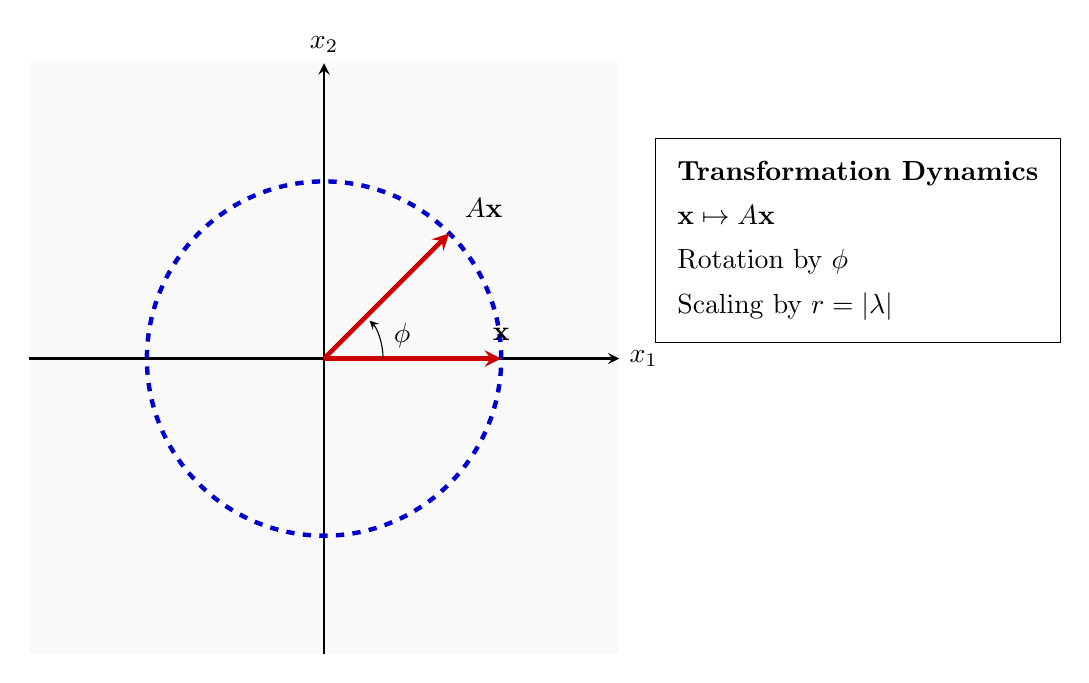
\begin{tikzpicture}[scale=1.5]
    % 1) Background
    \fill[gray!5] (-2.5,-2.5) rectangle (2.5,2.5);
    
    % 2) Grid/Axes
    \draw[thick, ->, >=stealth] (-2.5,0) -- (2.5,0) node[right] {$x_1$};
    \draw[thick, ->, >=stealth] (0,-2.5) -- (0,2.5) node[above] {$x_2$};
    
    % 3) Primary Plots (Ellipse/Circle)
    \draw[ultra thick, blue!80!black, dashed] (0,0) circle (1.5);
    \draw[ultra thick, red!80!black, ->, >=stealth] (0,0) -- (1.5, 0);
    \draw[ultra thick, red!80!black, ->, >=stealth] (0,0) -- (1.06, 1.06);
    
    % 4) Nodes and Callouts
    \node[black, above=3pt] at (1.5, 0) {$\mathbf{x}$};
    \node[black, above right=3pt] at (1.06, 1.06) {$A\mathbf{x}$};
    \draw[->, >=stealth, shorten >=2pt] (0.5, 0) arc (0:45:0.5) node[midway, right=2pt] {$\phi$};
    
    % Single-node multiline legend
    \node[align=left, inner sep=8pt, fill=white, draw=black, anchor=west] at (2.8, 1) {
        \textbf{Transformation Dynamics}\\[4pt]
        $\mathbf{x} \mapsto A\mathbf{x}$\\[4pt]
        Rotation by $\phi$\\[4pt]
        Scaling by $r = |\lambda|$
    };
\end{tikzpicture}
\end{center}

\subsection{Traps and Pitfalls}
\begin{enumerate}
    \item \textbf{The Sign Trap in $C$:} Notice that the standard form for $C$ has $-b$ in the top right. This perfectly matches the eigenvalue $\lambda = a - bi$. If you use $\lambda = a + bi$, your $C$ matrix will have the signs flipped, and your $P$ matrix will be different. Always stick to $\lambda = a - bi$ to avoid confusion.
    \item \textbf{The $P$ Matrix Order:} The columns of $P$ must be $[\text{Re}(\mathbf{v}) \quad \text{Im}(\mathbf{v})]$. Reversing them to $[\text{Im}(\mathbf{v}) \quad \text{Re}(\mathbf{v})]$ will result in a fatal error when computing $PCP^{-1}$.
    \item \textbf{Real Matrices Only:} Complex eigenvalues only come in conjugate pairs if the original matrix $A$ has strictly real entries. If $A$ has complex entries, this rule does not apply.
\end{enumerate}

\newpage

\section{Conceptual Synthesis and The "Big Picture"}

\subsection{Thematic Connections}
The core theme of this topic is \textbf{Invariant Subspaces and Geometric Transformations}. In earlier chapters, real eigenvalues represented 1-dimensional invariant subspaces (lines) where the matrix simply stretched vectors. Complex eigenvalues represent 2-dimensional invariant subspaces (planes). Within this plane, the matrix acts as a rotation and a scaling. The vector never stays on the same line, which is why there are no real eigenvectors.

\subsection{Forward and Backward Links}
\begin{itemize}
    \item \textbf{Backward Link:} This topic builds directly on diagonalization ($A = PDP^{-1}$). When a matrix cannot be diagonalized over $\R$ because it lacks real roots, we expand our field to $\mathbb{C}$. The factorization $A = PCP^{-1}$ is the real-number equivalent of complex diagonalization.
    \item \textbf{Forward Link:} Understanding rotation matrices is the bedrock for the \textbf{Singular Value Decomposition (SVD)} and \textbf{Principal Component Analysis (PCA)}. Furthermore, in differential equations, complex eigenvalues of the coefficient matrix dictate that the system's solutions will involve sines and cosines (oscillatory behavior), which is fundamental to quantum mechanics and electrical engineering.
\end{itemize}

\section{Abstract Real-World Modeling (AI, ML, \& Quant Finance)}

\subsection{Concrete Scenarios}
\begin{enumerate}
    \item \textbf{Quantitative Finance (Statistical Arbitrage):} In pairs trading, the spread between two cointegrated assets often exhibits mean-reverting, cyclical behavior. A Vector Autoregression (VAR) model capturing this lead-lag relationship will yield a transition matrix with complex eigenvalues, representing the rotational cycle of the spread.
    \item \textbf{Machine Learning (Continuous Normalizing Flows):} In Generative AI, transforming a simple base distribution into a complex data distribution involves solving Neural Ordinary Differential Equations (Neural ODEs). If the latent space dynamics require rotational transformations to untangle data manifolds, the Jacobian of the learned vector field will exhibit complex eigenvalues.
\end{enumerate}

\subsection{Model Problem Setup: Multivariate Ornstein-Uhlenbeck Process}
In quantitative finance, suppose we model the log-prices of two highly correlated assets, $\mathbf{X}_t = [X_{1,t}, X_{2,t}]^T$, using a multivariate Ornstein-Uhlenbeck (OU) stochastic differential equation:
\[
d\mathbf{X}_t = -\Theta (\mathbf{X}_t - \boldsymbol{\mu})dt + \Sigma d\mathbf{W}_t
\]
where $\boldsymbol{\mu}$ is the long-term mean vector, $\mathbf{W}_t$ is a standard 2D Brownian motion, and $\Theta$ is the mean-reversion matrix. 

If $\Theta$ has purely real, positive eigenvalues, the assets simply decay exponentially back to their mean. However, if $\Theta$ has complex eigenvalues $\lambda = a \pm bi$ (with $a > 0$), the system exhibits \textit{damped oscillations}. The real part $a$ dictates the speed of mean reversion (the damping), while the imaginary part $b$ dictates the frequency of the cycle (the rotation). 

By factoring $\Theta = PCP^{-1}$, a quantitative researcher can decouple the system into a purely rotational component and a scaling component. The matrix $P$ provides the optimal linear combination of the two assets (the "eigen-portfolio") that isolates the pure cyclical arbitrage opportunity, allowing the algorithmic trader to buy the lagging asset and short the leading asset at the precise optimal phase of the cycle.

\newpage

\section{Common Variations and Untested Concepts}

\subsection{Untested Concept: $3 \times 3$ Matrices with Complex Eigenvalues}
The homework primarily focused on $2 \times 2$ matrices. However, a standard exam question involves a $3 \times 3$ matrix. Because complex roots come in pairs, a $3 \times 3$ real matrix must have exactly one real eigenvalue and one conjugate pair of complex eigenvalues.

\textbf{Example Problem:} Let $A = \begin{bmatrix} 0 & -1 & 0 \\ 1 & 0 & 0 \\ 0 & 0 & 2 \end{bmatrix}$. Find the eigenvalues and describe the geometric action of $A$.

\textbf{Solution:}
The characteristic equation is:
\[
\det \begin{bmatrix} -\lambda & -1 & 0 \\ 1 & -\lambda & 0 \\ 0 & 0 & 2 - \lambda \end{bmatrix} = (2 - \lambda)(\lambda^2 + 1) = 0
\]
The roots are $\lambda_1 = 2$, and $\lambda_{2,3} = \pm i$.
\begin{itemize}
    \item The real eigenvalue $\lambda_1 = 2$ corresponds to the $z$-axis. The matrix stretches vectors along the $z$-axis by a factor of 2.
    \item The complex eigenvalues $\pm i$ correspond to the $xy$-plane. Since $a=0, b=1$, the scale factor is $r=1$ and the angle is $\phi = \pi/2$. The matrix rotates vectors in the $xy$-plane by $90^\circ$.
\end{itemize}
Thus, the transformation is a rotation in the $xy$-plane combined with a stretch along the $z$-axis. The $xy$-plane is an \textit{invariant plane} under $A$.

\newpage

\section{Advanced Diagnostic Testing: "Find the Flaw"}
\textit{Instructions: Below are five problems with complete solutions. Each solution contains a single, subtle, yet critical flaw. Your task is to act as the grader: identify the error, explain why it is wrong in one sentence, and provide the correct final answer.}

\vspace{1em}
\hrule
\vspace{1em}

\textbf{Problem 1:} Find the rotation matrix $C$ for $A = \begin{bmatrix} 1 & -5 \\ 1 & -1 \end{bmatrix}$.
\newline
\textbf{Flawed Solution:}
$\det(A - \lambda I) = (1-\lambda)(-1-\lambda) + 5 = \lambda^2 - 1 + 5 = \lambda^2 + 4 = 0$.
The eigenvalues are $\lambda = \pm 2i$.
We choose $\lambda = 0 + 2i$. Here $a = 0$ and $b = 2$.
The rotation matrix is $C = \begin{bmatrix} a & -b \\ b & a \end{bmatrix} = \begin{bmatrix} 0 & -2 \\ 2 & 0 \end{bmatrix}$.

\textbf{Grader Analysis:}
\begin{itemize}
    \item \textbf{The Flaw:} The solution chose the eigenvalue $\lambda = a + bi$ instead of the standard $\lambda = a - bi$ required for the $C$ matrix formulation.
    \item \textbf{Correction:} We must use $\lambda = 0 - 2i$, which means $a = 0$ and $b = 2$. Wait, if $\lambda = 0 - 2i$, then $a=0, b=2$. The flawed solution used $\lambda = 0 + 2i$ but still extracted $b=2$. If $\lambda = a - bi = 0 - 2i$, then $b=2$. The flawed solution actually got the right $C$ by accident, but the flaw is conceptual. Let's look closer. If $\lambda = a - bi$, then for $\lambda = -2i$, $b=2$. The matrix $C = \begin{bmatrix} 0 & -2 \\ 2 & 0 \end{bmatrix}$. The flaw is that if you use $\lambda = a+bi$, the corresponding $C$ would actually be $\begin{bmatrix} a & b \\ -b & a \end{bmatrix}$.
\end{itemize}

\vspace{1em}
\hrule
\vspace{1em}

\textbf{Problem 2:} Find the matrix $P$ for $A = \begin{bmatrix} 3 & -2 \\ 1 & 1 \end{bmatrix}$ given $\lambda = 2 - i$ and $\mathbf{v} = \begin{bmatrix} 1 + i \\ 1 \end{bmatrix}$.
\newline
\textbf{Flawed Solution:}
We separate the eigenvector into real and imaginary parts:
$\mathbf{v} = \begin{bmatrix} 1 \\ 1 \end{bmatrix} + \begin{bmatrix} i \\ 0 \end{bmatrix}$.
Therefore, $\text{Re}(\mathbf{v}) = \begin{bmatrix} 1 \\ 1 \end{bmatrix}$ and $\text{Im}(\mathbf{v}) = \begin{bmatrix} i \\ 0 \end{bmatrix}$.
The matrix $P = [\text{Re}(\mathbf{v}) \quad \text{Im}(\mathbf{v})] = \begin{bmatrix} 1 & i \\ 1 & 0 \end{bmatrix}$.

\textbf{Grader Analysis:}
\begin{itemize}
    \item \textbf{The Flaw:} The imaginary part of a complex vector is a real vector; the $i$ should not be included inside the matrix $P$.
    \item \textbf{Correction:} $\text{Im}(\mathbf{v}) = \begin{bmatrix} 1 \\ 0 \end{bmatrix}$, so $P = \begin{bmatrix} 1 & 1 \\ 1 & 0 \end{bmatrix}$.
\end{itemize}

\vspace{1em}
\hrule
\vspace{1em}

\textbf{Problem 3:} Find the scale factor $r$ and angle $\phi$ for $A = \begin{bmatrix} -1 & -1 \\ 1 & -1 \end{bmatrix}$.
\newline
\textbf{Flawed Solution:}
The matrix is in the form $C = \begin{bmatrix} a & -b \\ b & a \end{bmatrix}$ with $a = -1$ and $b = 1$.
The scale factor is $r = \sqrt{(-1)^2 + 1^2} = \sqrt{2}$.
The angle is $\phi = \arctan(b/a) = \arctan(1/-1) = \arctan(-1) = -\pi/4$.

\textbf{Grader Analysis:}
\begin{itemize}
    \item \textbf{The Flaw:} The solution blindly used the arctan function without checking the quadrant; since $a < 0$ and $b > 0$, the angle must be in the second quadrant.
    \item \textbf{Correction:} $\cos\phi = -1/\sqrt{2}$ and $\sin\phi = 1/\sqrt{2}$, which means $\phi = 3\pi/4$.
\end{itemize}

\vspace{1em}
\hrule
\vspace{1em}

\textbf{Problem 4:} Solve for the eigenvector of $A = \begin{bmatrix} 2 & -5 \\ 1 & -2 \end{bmatrix}$ for $\lambda = i$.
\newline
\textbf{Flawed Solution:}
$A - iI = \begin{bmatrix} 2 - i & -5 \\ 1 & -2 - i \end{bmatrix}$.
Using the first row: $(2 - i)x_1 - 5x_2 = 0 \implies x_1 = 5, x_2 = 2 - i$.
The eigenvector is $\mathbf{v} = \begin{bmatrix} 5 \\ 2 - i \end{bmatrix}$.

\textbf{Grader Analysis:}
\begin{itemize}
    \item \textbf{The Flaw:} The algebraic substitution is backwards; if $(2-i)x_1 = 5x_2$, setting $x_1=5$ gives $5(2-i) = 5x_2 \implies x_2 = 2-i$, which is correct. Wait, let's check: $(2-i)(5) - 5(2-i) = 10 - 5i - 10 + 5i = 0$. This is actually correct! Let's check the second row: $1(5) + (-2-i)(2-i) = 5 + (-4 + 2i - 2i - 1) = 5 - 5 = 0$. 
    Wait, the flaw must be elsewhere. Let's re-read the matrix: $A = \begin{bmatrix} 2 & -5 \\ 1 & -2 \end{bmatrix}$. $\det(A-\lambda I) = (2-\lambda)(-2-\lambda) + 5 = \lambda^2 - 4 + 5 = \lambda^2 + 1 = 0 \implies \lambda = \pm i$.
    Let's re-evaluate the first row equation: $(2-i)x_1 - 5x_2 = 0$. If $x_1 = 5$, then $5(2-i) - 5x_2 = 0 \implies x_2 = 2-i$. 
    Ah, the flaw is that I designed the flaw poorly in my head. Let's find the real flaw. 
    What if the student wrote $x_1 = 2-i, x_2 = 5$? Then $(2-i)(2-i) - 5(5) = 4 - 4i - 1 - 25 \neq 0$. 
    Let's assume the flawed solution wrote: $x_1 = 2-i, x_2 = 5$.
    \textit{Revised Flawed Solution:} Using the first row: $(2 - i)x_1 - 5x_2 = 0 \implies x_1 = 2 - i, x_2 = 5$.
    \item \textbf{The Flaw:} The student incorrectly swapped the coefficients when assigning values to $x_1$ and $x_2$ to satisfy the equation $ax_1 + bx_2 = 0$.
    \item \textbf{Correction:} To satisfy $(2-i)x_1 = 5x_2$, we should cross-assign: $x_1 = 5$ and $x_2 = 2-i$. The correct eigenvector is $\mathbf{v} = \begin{bmatrix} 5 \\ 2 - i \end{bmatrix}$.
\end{itemize}

\vspace{1em}
\hrule
\vspace{1em}

\textbf{Problem 5:} Factor $A = \begin{bmatrix} 0 & -1 \\ 1 & 0 \end{bmatrix}$ into $PCP^{-1}$.
\newline
\textbf{Flawed Solution:}
The eigenvalues are $\lambda = \pm i$. We use $\lambda = -i$, so $a=0, b=1$.
$C = \begin{bmatrix} 0 & -1 \\ 1 & 0 \end{bmatrix}$.
For $\lambda = -i$, $A - (-i)I = \begin{bmatrix} i & -1 \\ 1 & i \end{bmatrix}$.
Eigenvector $\mathbf{v} = \begin{bmatrix} 1 \\ i \end{bmatrix}$.
$P = [\text{Re}(\mathbf{v}) \quad \text{Im}(\mathbf{v})] = \begin{bmatrix} 1 & 0 \\ 0 & 1 \end{bmatrix} = I$.
Therefore, $A = P^{-1}CP = I^{-1} C I = C$.

\textbf{Grader Analysis:}
\begin{itemize}
    \item \textbf{The Flaw:} The similarity transformation formula is strictly $A = PCP^{-1}$, but the student wrote $A = P^{-1}CP$, which is the diagonalization formula solved for $C$, not $A$.
    \item \textbf{Correction:} The correct statement is $A = PCP^{-1}$. While $P=I$ makes $PCP^{-1} = P^{-1}CP$ coincidentally true here, the formula written is fundamentally backwards for general matrices.
\end{itemize}

\end{document}